\documentclass[11pt]{article}
\usepackage[margin=1in]{geometry}
\usepackage{booktabs}
\usepackage{graphicx}
\usepackage{microtype}
\usepackage[hidelinks]{hyperref}

\newcommand{\kZeroRecall}{0.88}
\newcommand{\kFourRecall}{0.92}
\newcommand{\kEightFaith}{0.94}


\title{\vspace{-2em}\textbf{Critique depth --- a documented near-null}}
\author{arxivkg · generation · critique depth}
\date{}

\begin{document}
\maketitle
\vspace{-2em}

\section*{What we did}
Vary only \texttt{critique\_k} $\in \{0, 4, 8\}$ --- the number of per-paper full-PDF critiques the
deep loop runs --- holding everything else constant, over the 27-topic battery. Scored on the metric
vector $+$ 4-axis judge $+$ faithfulness $+$ an order-debiased \textbf{pairwise} of \texttt{k8} vs
\texttt{k0}. The honest question: does reading more full PDFs measurably improve the review?

\section*{Results (mean over 27 topics)}
\begin{center}\begin{tabular}{lrrrrrrrrr}
\toprule
critique\_k & n critiques & words & num density & grounded & gold recall & j grounding & j coverage & j lineage & faithfulness \\
\midrule
k0 & 0.0 & 3026.0 & 35.6 & 45.88 & 0.88 & 5.0 & 4.56 & 5.0 & 0.99 \\
k4 & 3.38 & 3216.12 & 35.71 & 47.75 & 0.92 & 5.0 & 4.62 & 4.81 & 0.95 \\
k8 & 6.88 & 3027.25 & 36.5 & 43.5 & 0.88 & 4.88 & 4.44 & 4.81 & 0.94 \\
\bottomrule
\end{tabular}
\end{center}
\begin{center}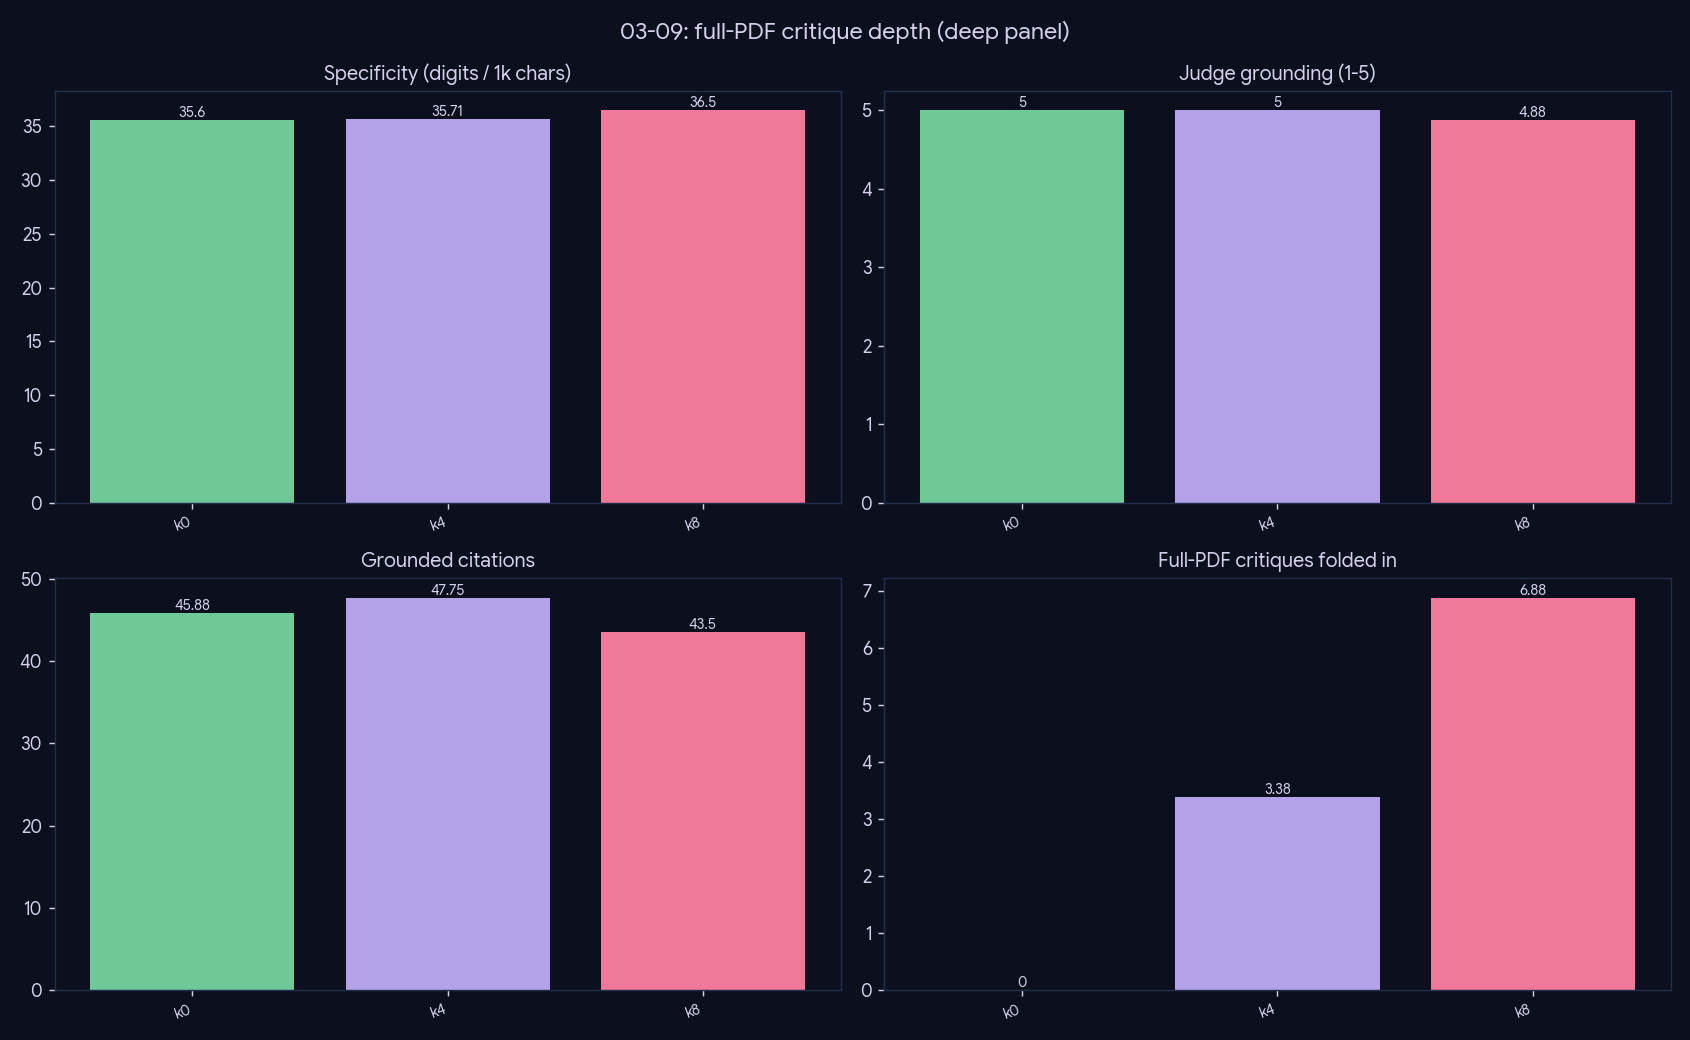
\includegraphics[width=0.95\textwidth]{../results/ablation.png}\end{center}

\section*{Conclusion}
\textbf{A documented near-null.} The first few critiques help a little --- gold recall
$\kZeroRecall\rightarrow\kFourRecall$ from \texttt{k0} to \texttt{k4} --- but \textbf{\texttt{k8} adds
nothing over \texttt{k4}} on recall or the judge, and faithfulness \emph{drops} (\kEightFaith{} at
\texttt{k8} vs 0.95 at \texttt{k0}): more critiqued passages give the composer more chances to
mis-attribute. The pairwise \texttt{k8} vs \texttt{k0} is a modest 0.63 overall --- below the deep
loop's 0.78 --- and is not backed by any objective-metric gain. \textbf{Critique depth is not a
quality lever beyond a handful}: keep \texttt{critique\_k} small ($\approx 4$); paying for $k=8$ buys
cost (full-PDF reads) and a faithfulness risk, not quality. \textbf{Caveat:} this is the kind of
honest null worth recording --- the deep loop's win (\texttt{03-08}) comes from the
\emph{retrieve-and-expand} rounds, not from critiquing more PDFs per round.

\end{document}
